\subsection{Topological Configurations of the \(\chi\) Field: Solitons as Particles}
  \label{app:topological_solitons}

  \paragraph{Status and scope of this construction.}
    The solitonic configurations discussed in this appendix are not introduced as
    fundamental degrees of freedom of Cosmochrony.
    They are \emph{effective geometric representations} intended to illustrate how
    particle-like properties may arise from stable, localized configurations of the
    \(\chi\) field \emph{once a smooth, orientable geometric projection becomes applicable}.

    At the fundamental level, Cosmochrony does not assume a pre-existing spatial
    manifold, metric, or differential structure.
    The scalar field \(\chi\) is not defined \emph{in} spacetime; rather, spacetime
    emerges as an effective description of relational regimes of \(\chi\).
    A fully relational and pre-geometric formulation is presented in
    Appendix~\ref{app:relational_formulation}.

    Throughout this appendix, all geometric notions (distance, rotation, circulation,
    surface integrals) refer exclusively to an \emph{effective projected field}
    \(\chi_{\mathrm{eff}}\), obtained once a stable projective regime is reached.
    None of the figures or constructions below should be interpreted as depicting
    the fundamental \(\chi\) field itself.

    Within this effective regime, particles are interpreted as
    \textbf{topologically stabilized solitonic configurations} of
    \(\chi_{\mathrm{eff}}\).
    Their apparent properties---such as \textbf{mass, spin, and charge}---do not
    correspond to independent fundamental quantum numbers, but emerge from the
    \textbf{structural organization and relaxation constraints} induced by these
    configurations.

\subsubsection{Charge as Oriented Relaxation Asymmetry of \(\chi_{\mathrm{eff}}\)}

  In Cosmochrony, electric charge is not associated with a fundamental gauge field,
  local symmetry, or conserved Noether current.
  Instead, it arises as an \emph{oriented asymmetry in the local relaxation structure}
  of the effective projected field \(\chi_{\mathrm{eff}}\).

  A localized solitonic configuration may deform the surrounding
  \(\chi_{\mathrm{eff}}\) profile in one of two qualitatively distinct ways:

  \begin{itemize}
    \item A \textbf{positive effective charge} corresponds to a \textbf{local excess}
    of \(\chi_{\mathrm{eff}}\) relative to its asymptotic background value
    \(\chi_{\mathrm{eff},0}\).
    Such configurations locally resist relaxation and generate repulsive relaxation
    gradients with similarly oriented deformations.
    \item A \textbf{negative effective charge} corresponds to a \textbf{local deficit}
    of \(\chi_{\mathrm{eff}}\) relative to \(\chi_{\mathrm{eff},0}\),
    favoring compensating relaxation and attractive interactions with oppositely
    oriented configurations.
  \end{itemize}

  This polarity does not reflect an intrinsic sign of \(\chi\) itself—which remains
  a scalar quantity without charge—but rather the orientation of the deformation
  with respect to the background relaxation flow in the projective regime.

  \paragraph{From structural asymmetry to observable charge.}
    Within an effective geometric description, the magnitude of the charge associated
    with a solitonic excitation is controlled by the \emph{net relaxation imbalance}
    induced by the configuration.

    This may be represented schematically by
    \[
      q_{\mathrm{eff}} \;\propto\;
      \int_{\Sigma}
      \bigl(\chi_{\mathrm{eff}} - \chi_{\mathrm{eff},0}\bigr)\, dS ,
    \]
    where \(\Sigma\) denotes a closed surface surrounding the localized configuration
    in effective space.
    This expression does not define a fundamental conserved quantity; it provides a
    coarse-grained measure of the structural asymmetry imposed on the relaxation of
    \(\chi_{\mathrm{eff}}\).

    In three effective spatial dimensions, the geometric dilution of the associated
    relaxation gradients naturally leads to inverse-square interaction laws.
    Coulomb-like behavior therefore emerges as a collective geometric response of
    \(\chi_{\mathrm{eff}}\), without introducing a fundamental electromagnetic field
    or gauge potential.

    \begin{figure}[h]
      \centering
      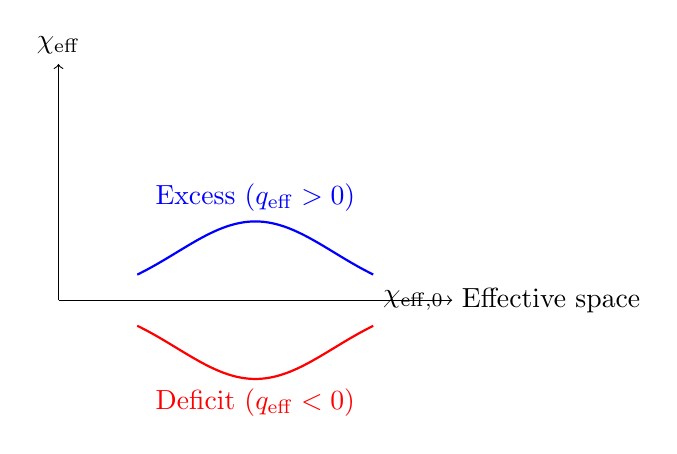
\begin{tikzpicture}[x=2cm, y=2cm]
        \draw[->] (0,0) -- (2.5,0) node[right] {Effective space};
        \draw[->] (0,0) -- (0,1.5) node[above] {$\chi_{\mathrm{eff}}$};

        \draw[thick, blue, domain=0.5:2, samples=100]
        plot (\x, {0.5*exp(-2*(\x-1.25)^2)});
        \node[blue, above] at (1.25, 0.5) {Excess ($q_{\mathrm{eff}}>0$)};

        \draw[thick, red, domain=0.5:2, samples=100]
        plot (\x, {-0.5*exp(-2*(\x-1.25)^2)});
        \node[red, below] at (1.25, -0.5) {Deficit ($q_{\mathrm{eff}}<0$)};

        \draw[dashed] (0.5,0) -- (2,0);
        \node[right] at (2,0) {$\chi_{\mathrm{eff},0}$};
      \end{tikzpicture}
      \caption{
        Schematic illustration of oriented deformations of the effective projected
        field \(\chi_{\mathrm{eff}}\).
        An excess or deficit relative to the background value
        \(\chi_{\mathrm{eff},0}\) determines the polarity of the effective charge.
        This diagram is purely illustrative and does not represent a solution of the
        fundamental \(\chi\) dynamics.
      }
      \label{fig:chi_charges}
    \end{figure}

\subsubsection{Vortical Configurations and Integer-Spin Excitations}
  \label{subsec:vortices}

  In the projectable regime, certain solitonic configurations of
  \(\chi_{\mathrm{eff}}\) admit cyclic internal organization patterns that can be
  described using an effective phase.
  When these patterns exhibit non-trivial circulation, the configuration may be
  modeled as a \emph{vortical soliton}.

  An effective winding number \(n\) may be defined as
  \[
    n = \frac{1}{2\pi}
    \oint \nabla \arg(\chi_{\mathrm{eff}}) \cdot d\mathbf{l},
  \]
  where all quantities refer to the emergent geometric representation.
  This winding number is not fundamental and has no meaning outside the projective
  regime.

  The integer \(n\) characterizes:
  \begin{itemize}
    \item the orientation of the relaxation asymmetry (sign of the effective charge),
    \item the topological robustness of the configuration,
    \item and the spin of the excitation, with integer values corresponding to
    bosonic behavior.
  \end{itemize}

  The energetic cost of such configurations increases with their internal structural
  complexity, leading to an effective mass scaling with \(|n|^2\) in minimal models.

  \begin{figure}[h]
    \centering
    \begin{tikzpicture}[x=2cm, y=2cm]
      \draw[->] (-1.5,0) -- (1.5,0) node[right] {$x$};
      \draw[->] (0,-1.5) -- (0,1.5) node[above] {$y$};

      \foreach \r in {0.2,0.4,...,1.2} {
        \draw[blue, thick, domain=0:6.28, samples=100]
        plot ({\r*cos(\x)}, {\r*sin(\x)});
      }

      \fill[red] (0,0) circle (0.05);
      \node[red, below] at (0,0) {Core};

      \node[blue] at (1.2,1.2) {$n=1$};
      \node[blue] at (1.2,0.8) {Integer spin};
    \end{tikzpicture}
    \caption{
      Illustrative vortical configuration of the effective field
      \(\chi_{\mathrm{eff}}\) with winding number \(n=1\).
      The circulation represents a cyclic relaxation pattern associated with
      integer spin.
      This figure is schematic and purely conceptual.
    }
    \label{fig:chi_vortex}
  \end{figure}

\subsubsection{Skyrmion-Like Configurations and Spin-\(\tfrac{1}{2}\) Excitations}
  \label{subsec:skyrmions}

  More complex solitonic configurations arise when the internal organization of
  \(\chi_{\mathrm{eff}}\) involves non-trivial mappings between internal orientation
  space and effective physical space.
  Such configurations may be modeled using skyrmion-like constructions.

  An effective topological index \(Q\) can be defined as
  \[
    Q = \frac{1}{4\pi}
    \int \mathbf{n} \cdot
    (\partial_x \mathbf{n} \times \partial_y \mathbf{n})\, dx\,dy ,
    \quad
    \mathbf{n} =
    \frac{\chi_{\mathrm{eff}}}{|\chi_{\mathrm{eff}}|}.
  \]

  Configurations with \(Q=\pm 1\) exhibit a characteristic
  \textbf{4\(\pi\)-periodicity} under rotations.
  A \(2\pi\) rotation does not return the configuration to an equivalent state,
  while a \(4\pi\) rotation does.
  This topological property provides a geometric origin for spin-\(\tfrac{1}{2}\)
  behavior and fermionic statistics within the projective regime.

  \begin{figure}[h]
    \centering
    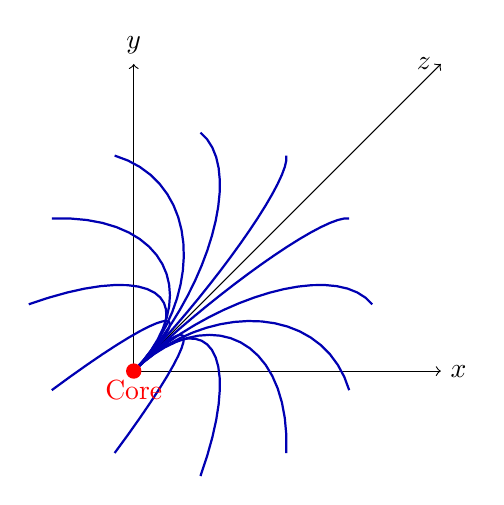
\begin{tikzpicture}[x=1.5cm, y=1.5cm, z=1.5cm, scale=1.3]
      \draw[->] (0,0,0) -- (2,0,0) node[right] {$x$};
      \draw[->] (0,0,0) -- (0,2,0) node[above] {$y$};
      \draw[->] (0,0,0) -- (0,0,2) node[left] {$z$};

      \foreach \phi in {0,30,...,330} {
        \draw[blue!70!black, thick, domain=0:1.2, samples=20]
        plot ({\x*sin(\x r)*cos(\phi)},
          {\x*sin(\x r)*sin(\phi)},
          {\x*cos(\x r)});
      }

      \fill[red] (0,0,0) circle (0.05);
      \node[red, below] at (0,0,0) {Core};
    \end{tikzpicture}
    \caption{
      Conceptual skyrmion-like configuration of \(\chi_{\mathrm{eff}}\),
      illustrating a spin-\(\tfrac{1}{2}\) excitation.
      The non-trivial internal mapping accounts for fermionic rotational behavior.
      This representation is purely illustrative.
    }
    \label{fig:chi_skyrmion}
  \end{figure}

\subsubsection{Summary: Topology, Charge, and Spin}

  \begin{table}[htbp]
    \centering
    \caption{Effective Solitonic Configurations and Emergent Particle Properties}
    \label{tab:solitons_charge}
    \begin{tabular}{|c|c|c|c|}
      \hline
      \textbf{Configuration} &
      \textbf{Topological Index} &
      \textbf{\(\chi_{\mathrm{eff}}\) Asymmetry} &
      \textbf{Emergent Properties} \\
      \hline
      Vortical soliton &
      Winding number \(n\) &
      Excess / deficit &
      Charge \(\propto n\), integer spin \\
      \hline
      Skyrmion-like soliton &
      Index \(Q=\pm1\) &
      Oriented deformation &
      Charge \(\propto Q\), spin-\(\tfrac{1}{2}\) \\
      \hline
    \end{tabular}
  \end{table}

  These constructions are not intended as a particle classification scheme nor as
  a replacement for the Standard Model.
  Their role is conceptual: to demonstrate how charge, mass, and spin may emerge
  coherently from the structural and topological organization of a single scalar
  substrate, without introducing additional fundamental fields, symmetries, or
  quantization postulates.
